\documentclass[handout]{beamer}
%\usepackage[margin=1in]{geometry}
\usepackage{amsthm,amsmath,amsfonts,hyperref,graphicx,color,multicol}
\usepackage{enumitem,tikz}

%%%%%%%%%%
%Beamer Template Customization
%%%%%%%%%%
\setbeamertemplate{navigation symbols}{}
\setbeamertemplate{theorems}[ams style]
\setbeamertemplate{blocks}[rounded]

\definecolor{Blu}{RGB}{43,62,133} % UWEC Blue
\setbeamercolor{structure}{fg=Blu} % Titles

%Unnumbered footnotes:
\newcommand{\blfootnote}[1]{%
	\begingroup
	\renewcommand\thefootnote{}\footnote{#1}%
	\addtocounter{footnote}{-1}%
	\endgroup
}


%%%%%%%%%%
%Custom Commands
%%%%%%%%%%
\newcommand{\R}{\mathbb{R}}
\newcommand{\veca}{\vec{a}}
\newcommand{\vecb}{\vec{b}}
\newcommand{\vece}{\vec{e}}
\newcommand{\vecu}{\vec{u}}
\newcommand{\vecv}{\vec{v}}
\newcommand{\vecw}{\vec{w}}
\newcommand{\vecx}{\vec{x}}
\newcommand{\zerovector}{\vec{0}}

\newcommand{\ds}{\displaystyle}

\newcommand{\fn}{\insertframenumber}

\newcommand{\rank}{\operatorname{rank}}
\newcommand{\adj}{\operatorname{adj}}

\newcommand{\blank}[1]{\underline{\hspace*{#1}}}


%%%%%%%%%%
%Custom Theorem Environments
%%%%%%%%%%
\theoremstyle{definition}
\newtheorem{exercise}{Exercise}
\newtheorem{question}[exercise]{Question}
\newtheorem*{defn}{Definition}
\newtheorem*{exa}{Example}
\newtheorem*{disc}{Group Discussion}
\newtheorem*{nb}{Note}
\newtheorem*{recall}{Recall}
\renewcommand{\emph}[1]{{\color{blue}\texttt{#1}}}

\definecolor{Gold}{RGB}{237, 172, 26}
%Statement block
\newenvironment{statementblock}[1]{%
	\setbeamercolor{block body}{bg=Gold!20}
	\setbeamercolor{block title}{bg=Gold}
	\begin{block}{\textbf{#1.}}}{\end{block}}


\begin{document}
	\title{Math 324: Linear Algebra}
	\subtitle{1.3: Applications of Systems of Linear Equations}
	\author{Mckenzie West}
	\date{Last Updated: \today}
\begin{frame}
\maketitle
\end{frame}

\begin{frame}{\insertframenumber}
	\begin{block}{\textbf{Last Time.}}
	\begin{itemize}[label=--]
		\item an algorithm for row reducing
		\item Gauss--Jordan elimination
		\item homogeneous equations
	\end{itemize}
	\end{block}
\begin{block}{\textbf{Today.}}
	\begin{itemize}[label=--]
		\item Polynomial curve fitting
		\item Network Analysis
	\end{itemize}
\end{block}
\end{frame}
\begin{frame}{\insertframenumber}
	\begin{recall}
		From the video for today, here is a fast and easy way to use SageMath to row reduce a matrix.
		
		Go to \url{http://sagecell.sagemath.org}.  
	
	Encode your matrix by row, then print out A along with its RREF:
	
	\texttt{A = matrix([[1,2,3,4],[5,6,7,8],[9,10,11,12]])\\
		print(A)\\
		print("The RREF of A")\\
		print(A.rref())\\}
	\end{recall}
\end{frame}
\begin{frame}{\insertframenumber}
	\begin{exa}[Polynomial Curve Fitting]
		When we have some data, we may want to approximate unknown data.
		One way to do this is to find a formula for a curve that passes through the points.
		
		Here is some sample data, the average high temperature in degrees Fahrenheit at the Gale Crater on Mars.
		
		\begin{center}
			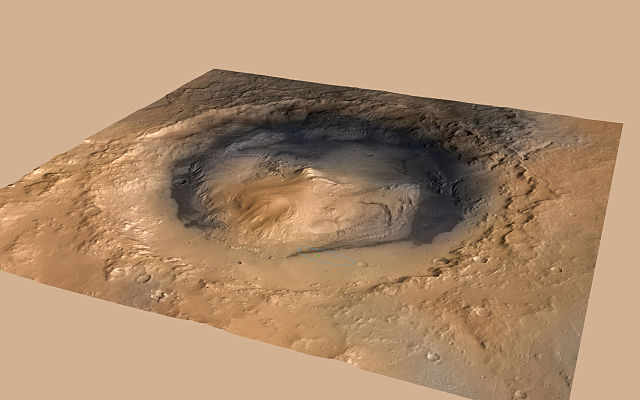
\includegraphics[width=1in]{images/Gale_Crater}
		\end{center}
		\[
			\begin{array}{r|ccc}
				\hline
				\textup{Month} & Jan & Mar & May\\
				\textup{Average High} & 19^{\circ } & -9^{\circ } & 25^{\circ }\\
				\hline
			\end{array}
		\]
	\end{exa}
	{\tiny Data acquired from \href{https://en.wikipedia.org/wiki/Climate_of_Mars}{Wikipedia: Climate of Mars}, accessed on 9/8/2019\\
	Image of Gale Crater also from Wikipedia}
\end{frame}

\begin{frame}{\insertframenumber}
\begin{exa}[Polynomial Curve Fitting Cont.]
	Let's encode the months at Jan = 1, Mar = 3, and May = 5.
	\[
	\begin{array}{r|ccc}
	\hline
	\textup{Month} & 1 & 3 & 5\\
	\textup{Average High} & 19^{\circ } & -9^{\circ } & 25^{\circ }\\
	\hline
	\end{array}
	\]
	Now we have have three points, $(1,19)$, $(3,-9)$ and $(5,25)$.
	
	With three points, we can construct a parabola (quadratic polynomial). 
	 
	If $f(x)=a+bx+cx^2$, then $a+b(1)+c(1)^2=19$, $a+b(3)+c(3)^2=-9$, and $a+b(5)+c(5)^2=25$.  
	
	Look! Three linear equations to be put into a matrix.
\end{exa}
\begin{exercise}
	Create a matrix to solve this linear system of equations.\pause
	
	Solve for $a,b$ and $c$.
%	\[\begin{bmatrix}
%		1&1&1&19\\
%		1&3&9&-9\\
%		1&5&25&25
%	\end{bmatrix}\longrightarrow
%	\begin{bmatrix}
%		1&0&0&225/4\\
%		0&1&0&-45\\
%		0&0&1&31/4
%	\end{bmatrix}\]
\end{exercise}
\end{frame}

\begin{frame}{\insertframenumber}
\begin{exercise}[Polynomial Curve Fitting Cont.]

Did you get: $a=225/4$, $b=-45$, and $c=31/4$?

If not, try again.
\pause

We can plot $y=a+bx+cx^2$ along with the original points:

\begin{center}
	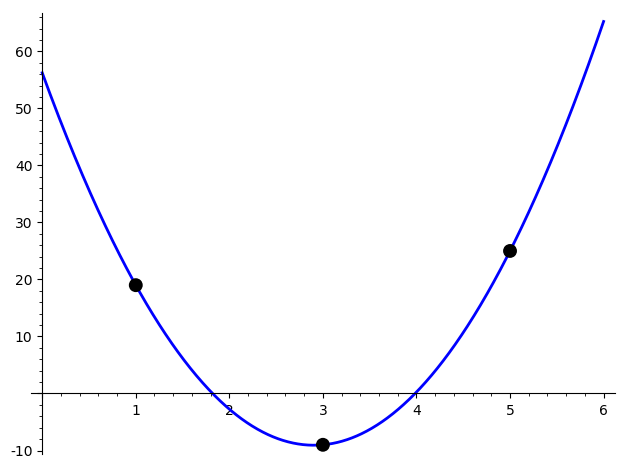
\includegraphics[width=1.75in]{images/mars_curve}
\end{center}

\end{exercise}
\end{frame}

\begin{frame}{\insertframenumber}
\begin{exercise}[Polynomial Curve Fitting Cont.]
\begin{enumerate}[label=(\alph*)]
	\item Approximate the average high temperature in February by plugging 2 in for $x$.
	\item The actual average temperature in February is $0^{\circ }$ Fahrenheit. Is your estimate close?
	\item Repeat this process for April.  The recorded average high temperature is $-4^{\circ }$F this month.
\end{enumerate}
\pause
See the plot below, with points indicating the actual recorded averages.
\begin{center}
	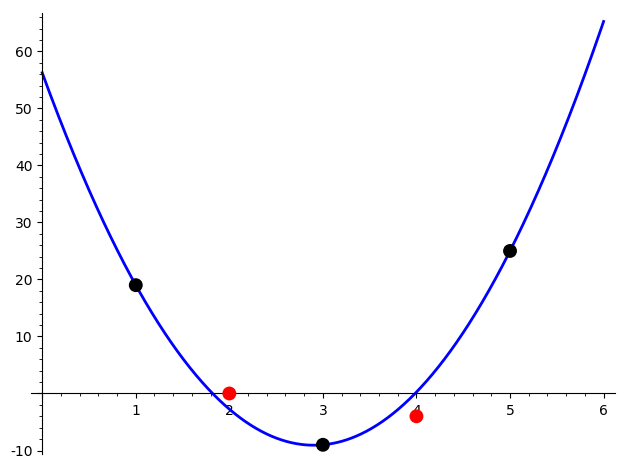
\includegraphics[width=1.75in]{images/mars_curve2}
\end{center}
\end{exercise}
\end{frame}

\begin{frame}{\insertframenumber}
\begin{exercise}[Polynomial Curve Fitting Cont.]
\[y=225/4-45x+31/4x^2\]

What is the approximation for the average high temperature in June?
%$f(6)=65.25$ 
\pause

The recorded average is 32.

See the plot below, with the green diamond indicating the actual recorded average in June.
\begin{center}
	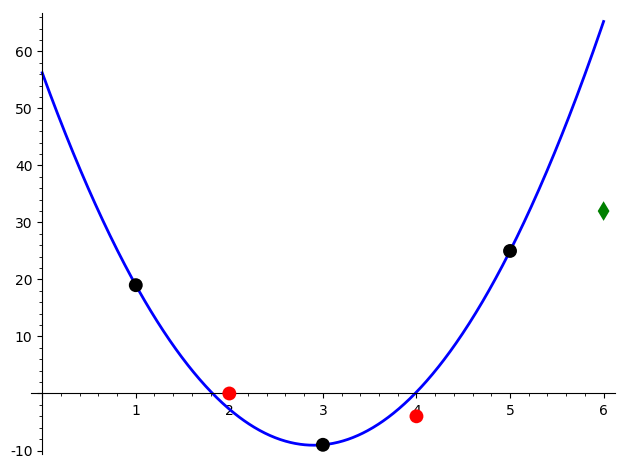
\includegraphics[width=1.75in]{images/mars_curve3}
\end{center}
\end{exercise}
\end{frame}

\begin{frame}{\insertframenumber}
\begin{question}
	Why is the estimate better for February and April than for June?
	
	What could you do to get better intermediate estimates?
\end{question}
\end{frame}

\begin{frame}{\fn}
	\begin{block}{\textbf{Brain Break.}}
		Remind your group members of your name.  Then share your answer to the following.
		
		What is the last movie you watched?
		
		\begin{center}
			
\includegraphics[width=2in]{images/camera}
		\end{center}
	\end{block}	
\end{frame}
\begin{frame}{\insertframenumber}
	\begin{exercise}
		The table shows the population size of Wisconsin for the years 1920, 1930, 1940, and 1950.  
		\vskip -.25in
		\[\begin{tabular}{r|cccc}
			\hline
			\textup{Year} & 1920&1930&1940&1950\\
			\textup{Population (in thousands)}&2632&2939&3137&3434\\
			\hline
		\end{tabular}\]
		
		\begin{enumerate}[label=(\alph*)]
			\item Use the data here to construct a cubic polynomial \[f(x)=a+bx+cx^2+dx^3\] approximating the number of people living in Wisconsin. 
			\item Approximate Wisconsin's population in 1935.
			\item Approximate Wisconsin's population in 2010.
		\end{enumerate}
	\end{exercise}
	{\tiny Data acquired from \href{http://worldpopulationreview.com/states/wisconsin-population/}{World Population Review}, accessed on 9/8/2019}
\end{frame}

\begin{frame}{\insertframenumber}
	\begin{exercise}
		The downtown core of Gotham City consists of one-way streets, and the traffic flow has been measured at each intersection.  For the city block shown in the following figure, the numbers represent the average numbers of vehicles per minute entering and leaving intersections $A,B,C$ and $D$ during business hours.
		
		Set up and solve a system of linear equations to find the possible flows $f_1,\dots,f_4$.
		
	\begin{minipage}{.5\textwidth}
		\begin{center}
		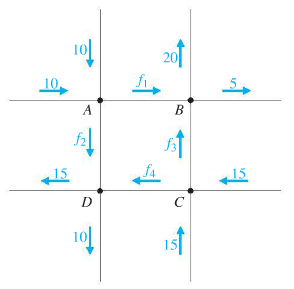
\includegraphics[height = 1.5in]{images/Gotham}
		\end{center}
	\end{minipage}
	\begin{minipage}{.4\textwidth}
	Note: At every intersection, the number of cars going in must equal the number of cars going out.
	\end{minipage}
	\end{exercise}
	{\tiny Exercise from Poole, David \textit{Linear Algebra: A Modern Introduction}, 4ed, Section 2.4}
\end{frame}

\begin{frame}{\insertframenumber}
	\begin{exercise}
		\begin{enumerate}[label=(\alph*)]
			\item If traffic is regulated on $CD$ so that $f_4=10$ vehicles per minute, what will the average flows on the other streets be?\pause
			\item What are the minimum and maximum possible flows on each street?\pause
			\item How would the solution change if \emph{all} of the directions were reversed?
		\end{enumerate}
	\end{exercise}
\end{frame}

\begin{frame}{\insertframenumber}
	\begin{exercise}
		The figure shows the boundary temperatures (in degrees Celcius) of an insulated thin metal plate.  The steady-state temperature of an interior junction is approximately equal to the mean of the temperatures at the four surrounding junctions.  Use a system of linear equations to approximate the interior temperatures $T_1,T_2,T_3$, and $T_4$.
	\begin{center}
		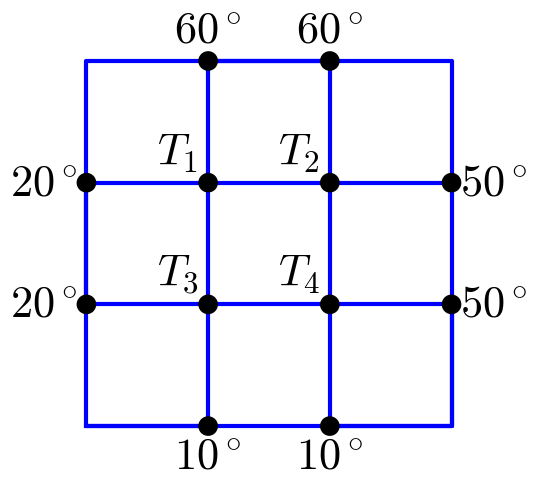
\includegraphics[width=2in]{images/temp_grid}
	\end{center}
	\end{exercise}
\end{frame}
\end{document}

